\chapter{Introduction}
\label{chap:introduction}
	
\begin{figure}[ht!]
  \begin{subfigure}[b]{0.5\textwidth}
	\centering\captionsetup{width=.9\linewidth}%
	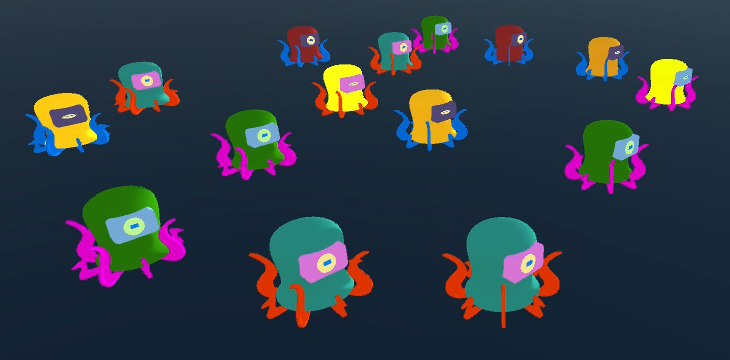
\includegraphics[width=\textwidth]{Assets/DocSegments/Chapters/Introduction/Figures/illustrative_system_result_figure_t1.png}
	\caption{Start of simulation. \tcol[white]{Her har jeg bare litt hvit tekst for å fylle inn.}}
	\label{fig:sub:illustrative_developed_system_t1}
  \end{subfigure}
  %
  \begin{subfigure}[b]{0.5\textwidth}
	\centering\captionsetup{width=.9\linewidth}%
	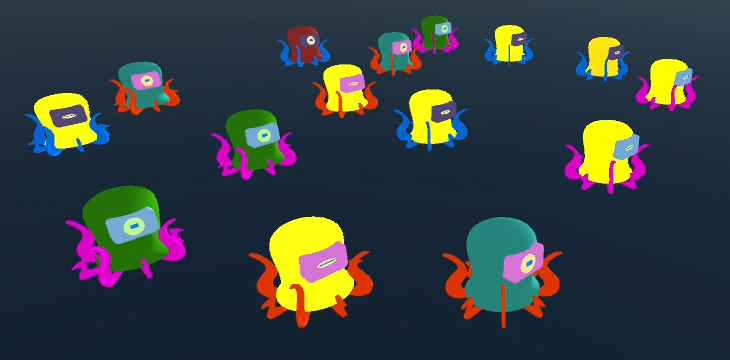
\includegraphics[width=\textwidth]{Assets/DocSegments/Chapters/Introduction/Figures/illustrative_system_result_figure_t2.png}
	\caption{Simulation at a later point in time than in \ref{fig:sub:illustrative_developed_system_t1}.}
	\label{fig:sub:illustrative_developed_system_t2}
  \end{subfigure}
  \begin{subfigure}[b]{0.5\textwidth}
	\centering\captionsetup{width=.9\linewidth}%
	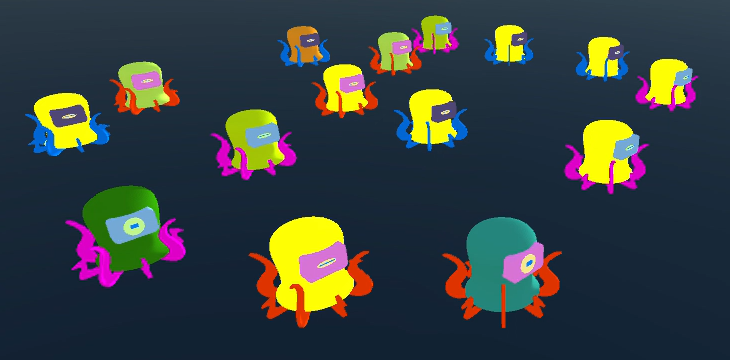
\includegraphics[width=\textwidth]{Assets/DocSegments/Chapters/Introduction/Figures/illustrative_system_result_figure_t3.png}
	\caption{Simulation at a later point in time than in \ref{fig:sub:illustrative_developed_system_t2}. \tcol[white]{Her har jeg bare litt hvit tekst for å fylle inn.}}
	\label{fig:sub:illustrative_developed_system_t3}
  \end{subfigure}
  %
  \begin{subfigure}[b]{0.5\textwidth}
	\centering\captionsetup{width=.9\linewidth}%
	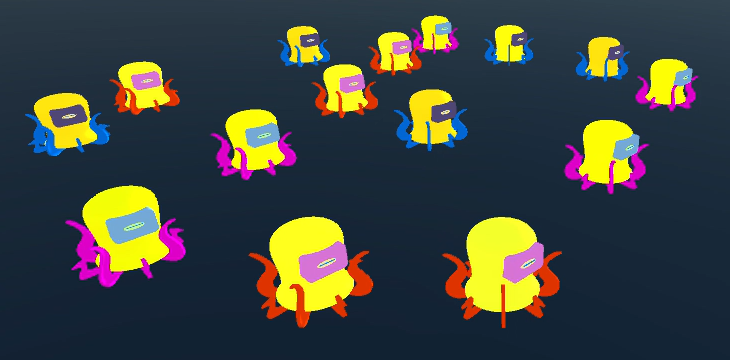
\includegraphics[width=\textwidth]{Assets/DocSegments/Chapters/Introduction/Figures/illustrative_system_result_figure_t4.png}
	\caption{Simulation at a later point in time than in \ref{fig:sub:illustrative_developed_system_t3}, around a minute later than in \ref{fig:sub:illustrative_developed_system_t1}.}
	\label{fig:sub:illustrative_developed_system_t4}
  \end{subfigure}
  \caption{A typical simulation run of a musical multi robot collective (here of size 15) entraining to achieve harmonic synchronization in the developed system. As we can see in \ref{fig:sub:illustrative_developed_system_t1}, the robots start flashing yellow and blinking with their eyes asynchronously, but end up synchronized in \ref{fig:sub:illustrative_developed_system_t4}.}
  \label{fig:illustrative_developed_system}
\end{figure}



\section{Motivation}

% Introducing challenges concerning knowledge and communication in (autonomous) computing systems given extreme and challenging environments:

Engineering a computing system for a certain environment often requires some knowledge of said environment; both on the end of the system-creator, as well as for the computing system in turn. This is at least the case in autonomous computing, where computing systems are supposed to be able to observe, learn, adapt, and act on their own, independently from their creator.

Foreseeing and predicting all possible (future) states and scenarios a computing system will face during its lifetime, in often extreme and complex, dynamic and ever-changing environments, at design-time is often hard, and sometimes impossible (in the case of coincidental faults e.g.). This calls for online and continuous learning at run time. If one wants to achieve coordination and continuous adaptation of a system or of system components (for example in a collective), some sort of intelligence might be necessary to endow it with.

Furthermore, extreme challenges and physical barriers within communication between decentralized and mobile robots and its human operator, like too large latencies, bottlenecks presented by using the same limited bandwidths, short possible ranges, or the inability to use global satellite systems e.g. in underwater vehicles \cite{petillot_underwater_robots}, leads to the necessity of enabling systems to autonomously and online control themselves and perform missions without communication from remote operators like humans. Hence, technological development and research has e.g. within underwater robotics gone from enabling remotely operated vehicles (ROVs) in the 1980s (for e.g. oil and gas exploitation at depths unreachable to human divers), over to more self adaptive and autonomous underwater vehicles (AUVs) closer to in the 21st century —the demand of which is expected to grow 37\% in the 2018-2022 period \cite{petillot_underwater_robots}. As a result, the underwater robots can in this instance thus, due to the increased degree of autonomy and consequently implicit reduction in communication need, travel on its own on even longer and extensive missions without the need for a live connection to any human operator—e.g. on seabed mapping missions, underwater machinery or structure maintenance, as well as seabed cleaning.

% Transitioning from autonomous agents to synchronizing oscillators:

However, and especially within collectives of multiple robots \cite{cocoro, swarm_bot}, communication between individuals—even though they might be autonomous individual robots—is still a challenge one has to deal with when designing them. Coordination, for humans and robots alike, often tend to demand a lot of communication. To add on top of this, when networks or collectives of sub-systems like wireless sensors are communicating with each other, they often have their own internal clock which often do not align. Hence, we see that both the magnitude of communication needed, as well as the inherent challenges with communication, call for effective approaches to communication with coordination as the goal.

As K. Konishi \& H. Kokame points out, one technical problem in e.g. wireless sensor networks is that each sensor node rely on accurate internal and synchronized clocks, especially from the perspective of sensor fusion and coordinating communication among nodes \cite{konishi_kokame}. Thus, time synchronization becomes recognized as one of the crucial problems in distributed and wireless systems \cite{tungvinte_sync_protocols}. Various attempts at synchronizing messages and communication, in order to e.g. align messages exchanged at unsynchronized intervals, has been made \cite{tungvinte_sync_protocols}; however, such attempts and protocols often require the computation of message exchange and processing, which wastes the limited computation capability of nodes and causes communication delays \cite{konishi_kokame}. To this, Konishi \& Kokame also point out how for synchronized pulse coupled oscillators (PCOs), such computation is not required. If internal clocks in communicating nodes are instead altered and synchronized to other nodes's clocks—instead of letting all clocks stay unsynchronized and constantly trying to compensate for this— it is rather apparent that getting rid of this need for compensation will considerably reduce computation needs while synchronized communication is still achieved.

Thus, by achieving time synchronization \cite{tungvinte_sync_protocols} through synchronizing pulse coupled oscillators, both the computational load, in addition to the need for communication, is considerably reduced; hence freeing up and saving valuable resources like e.g. processing power and energy (battery) in networks of individuals and possibly autonomous nodes, agents, or robots.


% SA + decentralized and autonomous (musical) robots / agents + Oscillator sync = <3 :

Self-awareness concepts from psychology are inspiring new approaches for engineering computing systems which operate in complex dynamic environments \cite{sacs16_ch2}. As we can see in various Music Technology Systems, this endowing can also give rise to interesting cooperative and coordinating behaviour.

With self awareness, online and continuous learning is achieved to a higher degree in contrast with other approaches (like ODA and MAPE-K), due to the limitations and downsides of these older approaches, as well as the advantages and upsides to considering computational self-awareness in computing systems. If one wants to achieve continuous adaptation of a system or of system-components (e.g. in a collective) — some sort of intelligence might be necessary to endow it with. Endowing computing systems with Self-Awareness can be beneficial in several respects, including but not limited to a greater capacity to adapt, to build potential for future adaptation in unknown environments, and to explain their behaviour to humans and other systems \cite{sacs17_ch3}.

Explainability has with time only become more and more relevant, also within artificial intelligence (AI) (hence the popularity of the term \textit{explainable AI}), as increasingly autonomous and automatically systems are making real life decisions with serious consequences increasingly on a day to day basis. L. A. Dennis and M. Fisher present explaining and verifiable agent-based systems, where rational agents who possess goals, beliefs, desires, intentions e.g. make decisions that in their opinion should be able to be questioned and giving an answer when prompted \cite{verifiable_and_questionable_agents}. Self awareness enables such questioning and answering by autonomous agents, as the agents themselves, since they are themselves aware of their knowledge, thoughts, goals, desires etc., can explain what lead to their actions. Or in other words, questions like ``what type of self awareness \cite{sacs16_ch2} (knowledge) lead to a certain self expression \cite{sacs16_ch2} (action)'' can be answered by self aware and self expressive agents. Such an example can be read by P. Lewis et al. \cite{sacs17_ch3} (3.3.4) when they summarize their novel computational self awareness framework by enabling self aware computing systems to produce sentences like the following: Peter (span) is aware of Ada's (scope) goal (aspect) to reduce the power usage (object). Further, Ada (span) is aware of her own reasoning (meta-self-awareness) about what to do (act) about it.

Endowing computing systems with Self-Awareness can be beneficial in several respects, including a greater capacity to adapt, to build potential for future adaptation in unknown environments, and to explain their behaviour to humans and other systems. As we can see in various Music Technology Systems, this endowing can also give rise to interesting cooperative and coordinating behaviour.

% --- \section END. ---



\section{Goal of the thesis} % a.k.a. research goals.

In this MSc-thesis, we will explore an exciting and relatively new translation of the concepts and notions regarding self-awareness — as they pertain to humans and animals especially — from the domain of Psychology, into the domain of computation and engineering. The problem to explore will mainly consist of studying the effects differing self-awareness levels, varying collective-sizes, levels of task difficulty (like more complex behaviours, and limited communication) - have on usefulness, system dynamics, overall performance, more intelligent systems, and scalability (in this case specifically within a musical robot system) when performing a task. Whether the effect of endowing the musical robot system with increased computational self awareness will be better decision making (or \textit{self expression} \cite{sacs16_ch2}), versatility and ability to adapt quickly and online in a rapidly dynamic and everchanging enviroment, as they continually learn by themselves further handling continuous environmental change, or not will be investigated.

Generally, the aim is to discover the effects of endowing computational systems/robots with self-awareness capabilities / abilities. More specifically, the aim of the thesis is to explore and investigate whether—and to which degrees—increased degree or level of computational self awareness in musical robots lead to increased performance in a collective musical task to be achieved; namely, achieving synchronization (\textit{harmonic} at that, cf. \ref{sec:harmonic_synchrony})—much like and inspired by fireflies in nature adjusting and synchronizing themselves and their flashing to each other.

With that, the following research questions is thus introduced, with the hope of answering them in the thesis: \nl

\textbf{Research Question 1}:

Will increased levels or degrees of computational self awareness in individual musical robots lead to the larger musical collective being able to achieve its musical collective task—being (\textit{harmonic}) synchronization—faster than with lower levels or degrees of computational self-awareness? \nl

\textbf{Research question 2}:

Can harmonic synchronization performance in a musical robot collective be maintained despite lower degrees or levels of computational self awareness? \nl

\textbf{Research Question 3}:

Will increased levels of self-awareness lead to more robustness and flexibility in terms of handling environmental noise and other uncertainties — specifically in the continued ability of musical robots to synchronize to each other efficiently despite these difficulties/challenges? \nl

% --- \section END. ---



\section{Outline}

The master's thesis is structured as follows. Firstly, past and related work relevant for the thesis will be presented in Chapter \ref{chap:background}, laying the theoretical and inspirational foundation this thesis is basing itself upon.

Then, in Chapter \ref{chap:baseline}, a particularly important and foundational approach to oscillator synchronization is presented in detail, serving as the starting point and baseline for the synchronization method the musical robots in our developed system will utilize in order to achieve the target state also presented and achieved by the authors of the baseline approach.

After the main specific approach of comparison and inspiration is presented in Chapter \ref{chap:baseline}, the specifics and details of the newly designed and implemented synchronization simulator will be expounded in Chapter \ref{chap:implementation}. Here, experimental setups will also be shown, for which we want to evaluate synchronization performance for in Chapter \ref{chap:experiments_and_results}. In this chapter, we will also analyze the experiments results from the motivated and set up experiments.

Finally, results found in Chapter \ref{chap:experiments_and_results} will be discussed and put into a broader context, as the thesis is concluded and discussed on a higher level, summarizing the whole thesis. Before references and eventual appendices are shown, possible future work as well as the main reasons why they were not possible to explore in the thesis work will be given.

% --- \section END. ---



\section{Contributions}

The main contributions this thesis work has led to is firstly that a novel synchronization simulator has been created and developed in Unity, where various and customly made synchronization methods can be implemented in a robot collective (either homogenously but also heterogenously in each robot); as well as that users of the simulator can both see and hear the robots's interactions and entrainment towards synchrony (including whether they manage to finally achieve synchrony, and in that case how long it takes them to get there). This novel framework opens, for everyone interested in it, for the possibility of experimenting with creative and novel synchronization-methods, in order to qualitatively and quantitatively assess their efficiency at achieving synchrony. A reason for this is due to the seamless scalability and dynamism, both in terms of robot-collective size, heterogenous or homogenous agents, as well as how a new update-function (for both phase updating and frequency updating) can so easily be added in and coded with a couple of lines.

The developed synchronization simulator in Unity, which is open to the world and those interested in it, serves as a testbed for seeing how changes in robots synchronizing affects synchronization performance; if e.g. someone thinks they have an idea for making the robots more clever, they can easily download the Unity simulator, implement their approach, and see analytical and graphical (as well as audible) results.

Differently than to earlier approaches to synchronizing pulsed coupled oscillators, and harmonically at that \cite{nymoen_synch}, the synchronization system developed in this thesis in Unity does not limit oscillator frequencies to stay within a certain range, and oscillator frequencies can both be adjusted to be larger than the max initial frequency, as well as smaller than the minimum initial frequency. In e.g. Nymoen et al.'s firefly inspired oscillator system, frequencies $\omega$ are limited to staying within the range of $[0.5Hz, 8Hz]$.

% --- \section END. ---